\chapter{Experimental Evaluation}
\label{chap:experiments}
This chapter evaluates the performance of the two solution
approaches developed in this thesis, namely the baseline
activity-oriented Relax-and-Fix (Chapter~\ref{chap:baseline})
and the group-based activity-oriented Relax-and-Fix
(Chapter~\ref{chap:grouprf}), on a standard set of benchmark
instances for the SAA-FSRCPSP\@. The evaluation is structured as
follows. Section~\ref{sec:setup} describes the benchmark
instances, parameter settings, and hardware environment.
Section~\ref{sec:baseline_vs_group} presents the head-to-head
comparison of the baseline and group-based approaches across
$n \in \{10, 30, 60, 120\}$ activities.
Section~\ref{sec:ablation} reports an ablation study on the
contribution of individual feature groups to clustering quality.
Section~\ref{sec:alpha_sensitivity} analyses the sensitivity
of the time aggregation factor~$\alpha$.
Section~\ref{sec:scen_red_exp} evaluates per-group scenario
reduction on the largest instance class.
Section~\ref{sec:discussion} discusses the findings and
identifies the conditions under which the group-based approach
offers the greatest benefit.
% ============================================================
\section{Experimental Setup}
\label{sec:setup}
% ============================================================
% ------------------------------------------------------------
\subsection{PSPLIB Instances}
\label{subsec:psplib}
% ------------------------------------------------------------
All experiments use instances drawn from the
\emph{Project Scheduling Problem Library}
(PSPLIB)~\parencite{Kolisch1997}, the standard
benchmark suite for resource-constrained project scheduling.
Four instance classes are considered.
\textbf{j10 instances.}
Each instance contains $n = 10$ real activities plus two dummy
activities (source and sink), for a total of 12 nodes in the
activity-on-node network. PSPLIB provides 480 j10 instances;
each resource-flexibility level $|K| \in \{1,2,3,4\}$ is
associated with 50 independent instances used here.
With $|S|=10$ SAA scenarios the resulting MIP model is
tractable within a few minutes on modern hardware
(see Table~\ref{tab:model_size} for detailed model dimensions).
\textbf{j30 instances.}
Each instance contains $n = 30$ real activities plus two dummy
nodes, for 32 activities in total.
PSPLIB provides 480 j30 instances; for each resource-flexibility
level $|K| \in \{1,2,3,4\}$, 50 instances are used
(Section~\ref{subsec:n30_results}).
With $|S|=10$ scenarios the resulting MIP model is substantially
larger than the j10 case (Table~\ref{tab:model_size}), making
individual solves considerably harder.
\textbf{j60 instances.}
Each instance contains $n = 60$ real activities plus two dummy
nodes, for 62 activities in total.
PSPLIB provides 480 j60 instances; for each $|K| \in \{1,2,3,4\}$,
50 instances are used (Section~\ref{subsec:n60_results}).
The j60 MIP models are too large to solve without time
aggregation ($\alpha \geq 5$); with aggregation, the effective
model size is comparable to j30 without aggregation.
\textbf{j120 instances.}
Each instance contains $n = 120$ real activities plus two dummy
nodes, for 122 activities in total.
PSPLIB provides 600 j120 instances; for each
$|K| \in \{1,2,3,4\}$, 50 instances are used
(Section~\ref{sec:scen_red_exp}).
At this scale, both time aggregation and per-group scenario
reduction are required for tractability.
In all four classes, renewable resource capacities and activity
durations are taken directly from the PSPLIB files. Stochastic
workloads $W_{isk}$ are generated by scaling the deterministic
resource requirements with independent draws from a
$\mathrm{Beta}(0.5,\,2.25)$ distribution, following the
parameterisation in Table~\ref{tab:params_exp}. A single
scenario set is drawn per instance and reused across both
methods.
% ------------------------------------------------------------
\subsection{Parameter Setting}
\label{subsec:params}
% ------------------------------------------------------------
Table~\ref{tab:params_exp} summarises all parameter settings
used throughout the experiments. Parameters are grouped into
three categories: SAA-FSRCPSP model parameters, solver
parameters, and grouping parameters specific to the group-based
approach.
\begin{table}[htbp]
\centering
\renewcommand{\arraystretch}{1.4}
\caption{Parameter settings for all experiments}
\label{tab:params_exp}
\begin{tabular}{llll}
\hline
\textbf{Category} &
\textbf{Parameter} &
\textbf{Value} &
\textbf{Description} \\
\hline
\multirow{4}{*}{SAA-FSRCPSP}
    & $|S|$         & 10              & Number of SAA scenarios \\
    & $\varepsilon$ & 0.1             & Violation tolerance \\
    & $CL$          & 0.9             & Confidence level \\
    & $f_i$         & $\beta[0.5, 2.25]$ & Workload scaling \\
\hline
\multirow{3}{*}{Solver}
    & $T_{\max}$     & see per-exp.\ table & Total time limit \\
    & $T_{\mathrm{model}}$ & see per-exp.\ table & Time limit per subproblem \\
    & MIP gap        & $10^{-5}$           & Optimality tolerance \\
\hline
\multirow{5}{*}{Grouping}
    & $\theta_{\mathrm{corr}}$    & 0.95 & Correlation pruning threshold \\
    & $\mathrm{min\_group\_size}$ & 1    & Minimum activities per group \\
    & $\mathrm{max\_group\_size}$ & see per-exp.\ table & Upper bound on group size \\
    & $\theta_{\mathrm{merge}}$   & 2.5  & Merge threshold (z-score) \\
    & $\eta$                      & 0    & Max non-improving groups \\
\hline
\end{tabular}
\end{table}
\noindent
The SAA scenario set for each instance is generated once and
kept fixed across all experiments, ensuring that solution
quality differences between approaches reflect algorithmic
differences rather than sampling variance. The MIP gap of
$10^{-5}$ ensures that all reported solutions are within
$0.001\%$ of optimality for the respective subproblem.
The per-subproblem time limit $T_{\mathrm{model}}$ is set
per experiment: 300\,s for j10 (EXP1) and 60\,s for j30
(EXP2). The j10 limit is generous because most j10 subproblems
close in under 30\,s; the 300\,s ceiling catches the rare
hard cases at $|K|=4$ without penalising the majority. For
j30, presolve and root-node processing alone consume a large
fraction of solver time, so 60\,s is chosen to allow at least
some branching while keeping the total experiment runtime
tractable across 50 instances.
% ------------------------------------------------------------
\subsection{Hardware}
\label{subsec:hardware}
% ------------------------------------------------------------
All experiments are conducted on a single machine with the
following configuration:
\begin{table}[htbp]
\centering
\renewcommand{\arraystretch}{1.4}
\caption{Hardware and software configuration}
\label{tab:hardware}
\begin{tabular}{ll}
\hline
\textbf{Component}    & \textbf{Specification} \\
\hline
Processor             & Apple M1 (ARM64), 8-core CPU \\
Physical cores        & 8 (performance + efficiency) \\
Memory                & 16\,GB unified memory \\
Operating system      & macOS Sonoma 14.x (Darwin 23.6.0) \\
\hline
Python version        & 3.11 \\
MIP solver            & Gurobi Optimizer 11.0.3 \\
                      & Academic licence (non-commercial) \\
Solver threads        & 4 (per subproblem) \\
Clustering library    & scikit-learn 1.4, SciPy 1.12 \\
\hline
\end{tabular}
\end{table}
\noindent
Gurobi is configured to use 4 of the 8 available logical
processors per subproblem, leaving the remaining 4 available
for the Python orchestration layer. All runtimes reported in
this chapter are wall-clock times measured in Python using
\texttt{time.time()}, accumulated over the MIP subproblem
solves. Feature extraction and grouping runtimes are not
included in the reported solve times, as they are negligible
($<0.1\,\text{s}$ per instance) compared to the MIP solve
times.
Gurobi runs as an x86\_64 binary under Rosetta~2 translation
on the ARM64 host, which may introduce a small overhead
relative to native x86\_64 hardware. Since both methods are
evaluated under identical conditions, relative comparisons
remain valid.
% ============================================================
\section{Results: Baseline vs.\ Group-based}
\label{sec:baseline_vs_group}
% ============================================================
% ------------------------------------------------------------
\subsection{\texorpdfstring{$n=10$}{n=10} Instances}
\label{subsec:n10_results}
% ------------------------------------------------------------
\subsubsection*{Experiment Configuration}
The j10 experiment compares both approaches across all four
resource-flexibility levels $|K| \in \{1,2,3,4\}$.
For each value of $|K|$, all 50 PSPLIB j10 instances are solved in two
sequential phases: Phase~1 runs the baseline on all 50
instances from a clean solver state, and Phase~2 runs the
group-based method on the same instances. This two-phase design
eliminates any warm-cache effects between methods. Both methods
receive the same SSGS warm-start $S_{\mathrm{SSGS}}$,
pre-computed once and cached before either phase begins.
Table~\ref{tab:exp1_params} lists the complete parameter
settings; values that differ from the general defaults in
Table~\ref{tab:params_exp} are marked with~$\dagger$.
\begin{table}[htbp]
\centering
\renewcommand{\arraystretch}{1.35}
\caption{EXP1 parameter settings (j10, $|K|=1\text{--}4$).
         Parameters that differ from the general setup
         (Table~\ref{tab:params_exp}) are marked with~$\dagger$.}
\label{tab:exp1_params}
\begin{tabular}{llll}
\hline
\textbf{Category} & \textbf{Parameter} & \textbf{Value} & \textbf{Note} \\
\hline
\multirow{3}{*}{SAA / Solver}
    & $|S|$                               & 10                    & Scenarios per instance \\
    & $T_{\max}$                          & $3{,}600\,\text{s}^\dagger$ & Total time limit \\
    & $T_{\mathrm{model}}$                & $300\,\text{s}^\dagger$     & Per-subproblem limit \\
    & $\varepsilon$                       & 0.1                   & Violation tolerance \\
\hline
\multirow{3}{*}{Baseline}
    & $\omega,\,\delta$                   & 1,\;0                 & Single-activity window \\
    & \texttt{max\_no\_improve}           & 0                     & No early stopping \\
\hline
\multirow{5}{*}{Group-based}
    & \texttt{max\_group\_size}           & $5^\dagger$           & Upper bound on group size \\
    & $\theta_{\mathrm{merge}}$           & 2.5                   & Merge threshold (z-score) \\
    & $\theta_{\mathrm{corr}}$            & 0.95                  & Redundancy pruning \\
    & \texttt{max\_no\_improve}           & 0                     & No early stopping \\
    & \texttt{stop\_on\_first\_feasible}  & \texttt{True}         & Halt after first feasible \\
\hline
\end{tabular}
\end{table}
\noindent
The per-subproblem limit of $T_{\mathrm{model}}=300\,\text{s}$
gives Gurobi ample time to close the gap on j10 subproblems,
which typically terminate in under 30\,s but can require
longer on the hardest $|K|=4$ instances. Setting
\texttt{max\_no\_improve}~$=0$ for both methods means neither
applies early stopping: the baseline iterates over every
activity and the group-based method processes every group,
regardless of whether the objective improves. With
\texttt{stop\_on\_first\_feasible}~$=\texttt{True}$, the
group-based method halts as soon as one integral feasible
solution is certified, rather than completing all groups.
\subsubsection*{Aggregate Results}
Table~\ref{tab:j10_summary} reports the aggregate performance
of both approaches across all four resource-flexibility levels.
For each $|K|$, the table shows feasibility rate, mean and
median wall-clock runtime, mean number of Fix-and-Relax
iterations (subproblems solved), and mean makespan gap relative
to the SSGS warm-start.
\begin{table}[htbp]
\centering
\renewcommand{\arraystretch}{1.35}
\caption{Aggregate results: j10 instances, 50 per $|K|$,
         $|S|=10$, $T_{\max}=3{,}600\,\text{s}$,
         $T_{\mathrm{model}}=300\,\text{s}$.}
\label{tab:j10_summary}
\begin{tabular}{c l r r r r r r}
\hline
\multirow{2}{*}{$|K|$} &
\multirow{2}{*}{\textbf{Method}} &
\textbf{Feas.} &
$\bar{t}$ &
$\tilde{t}$ &
$\bar{\iota}$ &
$\bar{\delta}$ &
\multirow{2}{*}{\textbf{Speedup}} \\
& & (/ 50) & (s) & (s) & & (\%) & \\
\hline
\multirow{2}{*}{1}
  & Baseline    & 50 & 112.5 & 33.0 & 2.92 & $-1.97$ & \multirow{2}{*}{$3.4\times$} \\
  & Group-based & 50 &  33.4 & 25.5 & 1.00 & $-1.97$ & \\
\hline
\multirow{2}{*}{2}
  & Baseline    & 50 & 176.4 & 71.2 & 1.84 & $-3.25$ & \multirow{2}{*}{$6.1\times$} \\
  & Group-based & 50 &  28.8 & 17.3 & 1.00 & $-3.66$ & \\
\hline
\multirow{2}{*}{3}
  & Baseline    & 50 & 137.6 & 31.0 & 2.22 & $-3.54$ & \multirow{2}{*}{$0.5\times$} \\
  & Group-based & 50 & 298.5 & 17.7 & 1.00 & $-2.88$ & \\
\hline
\multirow{2}{*}{4}
  & Baseline    & 43 & 796.3 & 90.9 & 4.64 & $-7.37$ & \multirow{2}{*}{$11.6\times$} \\
  & Group-based & \textbf{50} &  68.8 & 17.3 & 1.00 & $-8.11$ & \\
\hline
\end{tabular}
\end{table}
\subsubsection*{Feasibility}
At $|K| \in \{1,2,3\}$, both approaches solve all 50 instances
to feasibility. The differentiation appears at $|K|=4$,
where the baseline fails to certify a feasible integer solution
on 7 of the 50 instances within $T_{\max}$, while the
group-based method solves all~50. This difference arises because
the $|K|=4$ model has a much denser constraint structure: fixing
a single activity's variables per subproblem (baseline) produces
a weakly constrained relaxation that the MIP solver cannot
strengthen sufficiently within the per-subproblem budget.
Grouping all activities into a single cluster, as Ward
hierarchical clustering does uniformly for j10 instances
($\bar{m}=1.00$ groups across all~$|K|$), allows the solver to
explore the full combinatorial space of the instance in one
pass, recovering feasibility in all seven previously unsolvable
cases. The McNemar exact test confirms that this feasibility
advantage is statistically significant ($p = 0.016$).
\subsubsection*{Solution Quality}
Solution quality is measured as the percentage gap of the
returned makespan relative to the SSGS warm-start,
$\bar{\delta} = \overline{(z^* - z_{\mathrm{SSGS}})\,/\,
z_{\mathrm{SSGS}}} \times 100$.
Negative values indicate an improvement over the heuristic.
At $|K|=1$, both methods return identical makespans on every
instance (100\% tie rate), with a gap of $-1.97\%$.
At $|K|=2$, the group-based method wins on 2 instances and ties
on 48, achieving a slightly better mean gap ($-3.66\%$
vs.\ $-3.25\%$). At $|K|=3$, the picture is mixed: one instance
favours each method, with 48 ties; the baseline achieves a
marginally better mean gap ($-3.54\%$ vs.\ $-2.88\%$).
At $|K|=4$, of the 43 jointly feasible instances, 1 favours the
group-based method and 1 favours the baseline, with 41 ties.
The group-based method achieves a better mean gap ($-8.11\%$
vs.\ $-7.37\%$), partly because it certifies feasible
makespans on 7 instances where the baseline returns no solution.
The head-to-head breakdown is summarised in
Table~\ref{tab:j10_headtohead}.
\begin{table}[htbp]
\centering
\renewcommand{\arraystretch}{1.35}
\caption{Head-to-head solution quality: j10 instances.
         Counts refer to jointly feasible instances.}
\label{tab:j10_headtohead}
\begin{tabular}{c r r r r}
\hline
$|K|$ &
\textbf{Both feas.} &
\textbf{Grp wins} &
\textbf{Tie} &
\textbf{Base wins} \\
\hline
1 & 50 &  0 & 50 & 0 \\
2 & 50 &  2 & 48 & 0 \\
3 & 50 &  1 & 48 & 1 \\
4 & 43 &  1 & 41 & 1 \\
\hline
\end{tabular}
\end{table}
\subsubsection*{Runtime}
The group-based approach is faster at $|K| \in \{1,2,4\}$ but
slower at $|K|=3$ in terms of mean runtime. At $|K|=1$ and
$|K|=2$, speedups of $3.4\times$ and $6.1\times$ are observed.
At $|K|=4$, where the baseline wastes time on 7 infeasible
instances that each run to the time limit, the speedup reaches
$11.6\times$.
At $|K|=3$, the group-based mean runtime of 298.5\,s exceeds
the baseline's 137.6\,s (speedup $= 0.5\times$). This is
caused by a single outlier instance whose group-based solve
reaches 2\,148\,s. The median runtime tells a different story:
17.7\,s for the group-based method versus 31.0\,s for the
baseline, confirming that the group-based method is faster on
the typical instance even at $|K|=3$.
The primary driver of the speedup is the iteration count: Ward
hierarchical clustering collapses all j10 activities into a
single group ($\bar{\iota}^{\mathrm{grp}} = 1.0$ for
all~$|K|$), so the group-based method solves a single
subproblem per instance rather than iterating
activity-by-activity. The baseline requires 2--5 subproblem
solves on average ($\bar{\iota}^{\mathrm{base}} = 2.92$ at
$|K|=1$, rising to 4.64 at $|K|=4$), each allocated up to
$T_{\mathrm{model}}=300\,\text{s}$.
Figure~\ref{fig:j10_comparison} visualises these trends.
\begin{figure}[htbp]
  \centering
  
\includegraphics[width=\textwidth]{figures/exp1_10_j10_figure.png}
  \caption{Experiment~1: j10 instances ($|S|=10$, 50 per $|K|$).
           \textbf{(A)}~Feasibility rate.
           \textbf{(B)}~Mean makespan (feasible instances only).
           \textbf{(C)}~Mean runtime with speedup annotations.
           \textbf{(D)}~Mean gap vs.\ SSGS (negative =
           improvement). SSGS shown as green reference line.}
  \label{fig:j10_comparison}
\end{figure}
% ============================================================
% Section 7.2.2  –  n = 30 Instances  (j30, |K| = 1..4)
% Source: EXP2_sil030_fixed_merge/exp2_j30_k{1..4}.csv
% ============================================================
\subsection{\texorpdfstring{$n=30$}{n=30} Instances}
\label{subsec:n30_results}
\subsubsection*{Experiment Configuration}
The j30 experiment compares both approaches across all four
resource-flexibility levels $|K| \in \{1,2,3,4\}$, mirroring
the j10 design. For each value of $|K|$, the 50 PSPLIB j30
instances are
solved in two sequential phases: Phase~1 runs the baseline on
all 50 instances from a clean solver state, and Phase~2 runs the
group-based method on the same instances. Both methods receive
the same SSGS warm-start $S_{\mathrm{SSGS}}$, pre-computed once
and cached before either phase begins.
Table~\ref{tab:exp2_params} lists the experiment-specific
parameter settings.
\begin{table}[ht]
\centering
\renewcommand{\arraystretch}{1.35}
\caption{EXP2 parameter settings (j30, $|K|=1\text{--}4$).
         Parameters that differ from the general setup
         (Table~\ref{tab:params_exp}) are marked with~$\dagger$.}
\label{tab:exp2_params}
\begin{tabular}{llll}
\hline
\textbf{Category} & \textbf{Parameter} & \textbf{Value} & \textbf{Note} \\
\hline
\multirow{3}{*}{SAA / Solver}
    & $|S|$                               & 10                    & Scenarios per instance \\
    & $T_{\max}$                          & $3{,}600\,\text{s}^\dagger$ & Total time limit \\
    & $T_{\mathrm{model}}$                & 60\,s                 & Per-subproblem limit \\
\hline
\multirow{2}{*}{Baseline}
    & $\omega,\,\delta$                   & 1,\;0                 & Single-activity window \\
    & \texttt{max\_no\_improve}           & 0                     & No early stopping \\
\hline
\multirow{5}{*}{Group-based}
    & \texttt{max\_group\_size}           & $10^\dagger$          & Produces 2--3 groups for j30 \\
    & $\theta_{\mathrm{merge}}$           & 2.5                   & Merge threshold \\
    & $\theta_{\mathrm{corr}}$            & 0.95                  & Redundancy pruning \\
    & \texttt{max\_no\_improve}           & 0                     & No early stopping \\
    & \texttt{stop\_on\_first\_feasible}  & \texttt{True}         & Halt after first feasible \\
\hline
\end{tabular}
\end{table}
\noindent
Setting \texttt{max\_group\_size}~$=10$ allows the grouper to
form larger, fewer groups on j30 instances ($n=30$), typically
resulting in 2--3 groups per instance. With
\texttt{stop\_on\_first\_feasible}~$=\texttt{True}$, the
group-based method halts as soon as one integral feasible
solution is certified, focusing computational effort on
feasibility rather than continued makespan improvement.
\subsubsection*{Aggregate Results}
Table~\ref{tab:j30_summary} reports the aggregate performance
of both approaches across all four resource-flexibility levels.
For each $|K|$, the table shows feasibility rate, mean
wall-clock runtime, mean number of Fix-and-Relax iterations
(subproblems solved), mean makespan gap relative to the SSGS
warm-start, and the runtime speedup.
\begin{table}[htbp]
\centering
\renewcommand{\arraystretch}{1.35}
\caption{Aggregate results: j30 instances, 50 instances per $|K|$,
         $|S|=10$ scenarios, $T_{\max}=3{,}600\,\text{s}$,
         $T_{\mathrm{model}}=60\,\text{s}$.
         \emph{Feas.}: feasible instances of 50;
         $\bar{t}$: mean runtime (s);
         $\tilde{t}$: median runtime (s);
         $\bar{\iota}$: mean Fix-and-Relax iterations;
         $\bar{\delta}$: mean gap vs.\ SSGS (\%).
         Speedup $= \bar{t}^{\,\mathrm{base}} /
         \bar{t}^{\,\mathrm{grp}}$.}
\label{tab:j30_summary}
\begin{tabular}{c l r r r r r r}
\hline
\multirow{2}{*}{$|K|$} &
\multirow{2}{*}{\textbf{Method}} &
\textbf{Feas.} &
$\bar{t}$ &
$\tilde{t}$ &
$\bar{\iota}$ &
$\bar{\delta}$ &
\multirow{2}{*}{\textbf{Speedup}} \\
& & (/ 50) & (s) & (s) & & (\%) & \\
\hline
\multirow{2}{*}{1}
  & Baseline    & 35 & 541.3 &  56.7 & 19.6 & $-0.12$ & \multirow{2}{*}{$5.4\times$} \\
  & Group-based & \textbf{39} & 100.1 &  51.8 &  1.8 & $-0.83$ & \\
\hline
\multirow{2}{*}{2}
  & Baseline    & 38 & 656.5 &  60.4 & 15.7 & $-0.03$ & \multirow{2}{*}{$4.1\times$} \\
  & Group-based & \textbf{40} & 160.2 &  60.3 &  2.0 & $-0.09$ & \\
\hline
\multirow{2}{*}{3}
  & Baseline    & 31 & 1{,}477.2 & 182.6 & 25.3 & $-0.04$ & \multirow{2}{*}{$5.1\times$} \\
  & Group-based & \textbf{32} &   288.2 &  60.5 &  2.8 & $-0.04$ & \\
\hline
\multirow{2}{*}{4}
  & Baseline    & \textbf{28} & 1{,}746.8 & 1{,}301.4 & 27.5 & $0.00$ & \multirow{2}{*}{$4.7\times$} \\
  & Group-based & 26 &   368.1 &   246.7 &  3.1 & $0.00$ & \\
\hline
\end{tabular}
\end{table}
\subsubsection*{Feasibility}
Unlike the j10 case, feasibility on j30 instances is far from
guaranteed. At $|K| \in \{1,2,3\}$, the group-based approach
finds more feasible solutions than the baseline:
$78\%$ vs.\ $70\%$ at $|K|=1$, $80\%$ vs.\ $76\%$ at $|K|=2$,
and $64\%$ vs.\ $62\%$ at $|K|=3$. In every case the set of
baseline-feasible instances is a \emph{subset} of the
group-based feasible instances; that is, the group-based
method solves everything the baseline solves plus 4, 2, and 1
additional instances at $|K|=1,2,3$ respectively.
At $|K|=4$ the picture is different: the baseline finds 28
feasible solutions versus 26 for the group-based method. The
two instances solved only by the baseline are cases where the
per-subproblem limit of $T_{\mathrm{model}}=60\,\text{s}$ is
too tight for the larger group subproblems at this constraint
density. Either way, neither method exceeds $56\%$ feasibility
at $|K|=4$, which underlines how hard the j30 model becomes
with $|S|=10$ scenarios and 4 resource types.
\subsubsection*{Solution Quality}
Table~\ref{tab:j30_headtohead} summarises the head-to-head
comparison on instances where both methods found a feasible
solution.
\begin{table}[htbp]
\centering
\renewcommand{\arraystretch}{1.35}
\caption{Head-to-head solution quality: j30 instances.
         Counts refer to instances where both methods found a
         feasible solution.}
\label{tab:j30_headtohead}
\begin{tabular}{c r r r r}
\hline
$|K|$ &
\textbf{Both feas.} &
\textbf{Grp wins} &
\textbf{Tie} &
\textbf{Base wins} \\
\hline
1 & 35 & 4 & 30 & 1 \\
2 & 38 & 1 & 37 & 0 \\
3 & 31 & 0 & 31 & 0 \\
4 & 26 & 0 & 26 & 0 \\
\hline
\end{tabular}
\end{table}
At $|K|=1$, the group-based approach strictly improves over the
baseline on 4 of 35 jointly feasible instances, with the most
notable improvement on \texttt{j309\_2} where the makespan drops
from 100 (baseline = SSGS warm-start) to 80, a gain of 20
time units ($-20\%$). At $|K|=2$, one instance
(\texttt{j3018\_8}) is strictly improved from 88 to 86.
At $|K| \in \{3,4\}$, both methods return identical makespans on
all jointly feasible instances, with gaps very close to zero,
indicating that the SSGS warm-start already provides a strong
solution at higher resource counts. The baseline wins on only 1
instance across all 130 jointly feasible comparisons ($<1\%$).
\subsubsection*{Runtime}
Across all four resource-flexibility levels, the group-based
approach is $4$--$5\times$ faster than the baseline. The reason
is straightforward: the baseline requires 16--28 Fix-and-Relax
iterations on average (one per activity), while the group-based
method completes in 2--3 iterations (one per cluster). At
$|K|=4$, the mean baseline runtime reaches 1{,}747\,s (nearly
30 minutes), whereas the group-based method finishes in 368\,s.
The median runtimes tell a similar story: at $|K|=3$, the
baseline median is 182.6\,s compared to 60.5\,s for the
group-based method, so the speedup is not simply caused by a
few outlier instances. Figure~\ref{fig:j30_comparison} visualises these trends.
\begin{figure}[htbp]
  \centering
  
\includegraphics[width=\textwidth]{figures/exp2_j30_figure.pdf}
  \caption{Experiment~1: j10 instances ($|S|=10$, 50 per $|K|$).
           \textbf{(A)}~Feasibility rate.
           \textbf{(B)}~Mean makespan (feasible instances only).
           \textbf{(C)}~Mean runtime with speedup annotations.
           \textbf{(D)}~Mean gap vs.\ SSGS (negative =
           improvement). SSGS shown as green reference line.}
  \label{fig:j30_comparison}
\end{figure}
\subsubsection*{Results with Time Aggregation ($\alpha = 2$)}
As Table~\ref{tab:j30_summary} shows, without time aggregation
both methods leave a large fraction of j30 instances unsolved,
especially at $|K| \geq 3$ where more than one-third remain
infeasible. Applying even modest time aggregation with
$\alpha = 2$ (halving the time horizon) changes the situation
considerably. Table~\ref{tab:j30_alpha2} reports the results of
the group-based R\&F with $\alpha = 2$ on the same 50 instances
per $|K|$.
\begin{table}[htbp]
\centering
\renewcommand{\arraystretch}{1.35}
\caption{Group-based R\&F with time aggregation ($\alpha=2$):
         j30 instances, 50 per $|K|$, $|S|=10$.
         \emph{Feas.}: feasible instances of 50;
         $\bar{\delta}$: mean gap vs.\ SSGS~(\%);
         Impr.: instances strictly improved over SSGS;
         $\bar{t}$: mean MIP solve time~(s);
         $\bar{m}$: mean groups formed.}
\label{tab:j30_alpha2}
\begin{tabular}{c r r r r r}
\hline
$|K|$ &
\textbf{Feas.} (/ 50) &
$\bar{\delta}$ (\%) &
\textbf{Impr.} &
$\bar{t}$ (s) &
$\bar{m}$ \\
\hline
1 & \textbf{50} & $-1.15$ & 25 & 31.9 & 1.00 \\
2 & \textbf{50} & $-0.12$ & 20 & 43.6 & 1.00 \\
3 & 49 & $-1.54$ & 27 & 55.3 & 1.20 \\
4 & 46 & $-0.26$ & 20 & 98.0 & 1.52 \\
\hline
\end{tabular}
\end{table}
Feasibility jumps at every resource-flexibility level: from
$78\%$ to $100\%$ at $|K|=1$, from $80\%$ to $100\%$ at
$|K|=2$, from $64\%$ to $98\%$ at $|K|=3$, and from $52\%$ to
$92\%$ at $|K|=4$. What is perhaps more interesting is that the
mean SSGS gap is \emph{negative} at all four levels: the MIP
solver actually \emph{improves} on the heuristic warm-start on
average, by $-1.15\%$ at $|K|=1$ and $-1.54\%$ at $|K|=3$.
Between $40\%$ and $54\%$ of instances end up with a makespan
strictly below the SSGS warm-start, with the best individual
improvement reaching $-23.7\%$. Runtimes drop as well:
$32$--$98\,\text{s}$ on average versus $100$--$368\,\text{s}$
without aggregation, since the compressed time horizon reduces
the number of variables and constraints in each subproblem.
In short, even a moderate aggregation factor of $\alpha = 2$ is
enough to make j30 instances tractable for the group-based
R\&F while maintaining (or improving) solution quality relative
to the SSGS heuristic. Figure~\ref{fig:j30_alpha2} summarises
these results visually, and Figure~\ref{fig:j30_comparison}
visualises the baseline-vs-grouped comparison without
aggregation.
\begin{figure}[htbp]
  \centering
  
\includegraphics[width=\textwidth]{figures/exp7_j30_alpha2_figure.pdf}
  \caption{Group-based R\&F with time aggregation ($\alpha=2$)
           on j30 instances ($|S|=10$, 50 instances per~$|K|$).
           \textbf{(A)}~Feasibility rate.
           \textbf{(B)}~Mean makespan gap relative to the
           SSGS warm-start (negative~=~improvement).
           \textbf{(C)}~Number of instances with makespan
           strictly below the SSGS warm-start.
           \textbf{(D)}~Mean wall-clock runtime.}
  \label{fig:j30_alpha2}
\end{figure}
% ============================================================
% Section 7.2.3  –  n = 60 Instances  (j60, |K| = 1..4)
% Source: EXP5/exp5_j60_k{1..4}_alpha{5,7}.csv
% ============================================================
\subsection{\texorpdfstring{$n=60$}{n=60} Instances}
\label{subsec:n60_results}
\subsubsection*{Experiment Configuration}
At $n=60$ activities the SAA-FSRCPSP model without time
aggregation is too large for either method to solve within a
tractable time budget (cf.\ Section~\ref{sec:alpha_sensitivity}).
The j60 experiment therefore evaluates the group-based R\&F with
time aggregation, using $\alpha = 5$ for $|K| \in \{1,2\}$ and
$\alpha = 7$ for $|K| \in \{3,4\}$, which are the smallest values that
achieve 100\% feasibility in the sensitivity analysis. Since the
baseline activity-oriented R\&F does not incorporate time
aggregation, this experiment reports only the group-based method.
For each $|K|$, 50 PSPLIB j60 instances are solved with
$|S| = 10$ scenarios, $T_{\mathrm{model}} = 60\,\text{s}$, and
$T_{\max} = 600\,\text{s}$. Table~\ref{tab:exp3_params} lists
the experiment-specific settings.
\begin{table}[htbp]
\centering
\renewcommand{\arraystretch}{1.35}
\caption{EXP3 parameter settings (j60, $|K|=1\text{--}4$).
         Parameters that differ from the general setup
         (Table~\ref{tab:params_exp}) are marked with~$\dagger$.}
\label{tab:exp3_params}
\begin{tabular}{llll}
\hline
\textbf{Category} & \textbf{Parameter} & \textbf{Value} & \textbf{Note} \\
\hline
\multirow{4}{*}{SAA / Solver}
    & $|S|$                               & 10                     & Scenarios per instance \\
    & $T_{\max}$                          & $600\,\text{s}^\dagger$ & Total time limit \\
    & $T_{\mathrm{model}}$                & 60\,s                  & Per-subproblem limit \\
    & $\alpha$                            & $5$ / $7^\dagger$      & Time aggregation factor \\
\hline
\multirow{5}{*}{Group-based}
    & \texttt{max\_group\_size}           & $10$                   & Upper bound on group size \\
    & $\theta_{\mathrm{merge}}$           & 2.5                    & Merge threshold \\
    & $\theta_{\mathrm{corr}}$            & 0.95                   & Redundancy pruning \\
    & \texttt{max\_no\_improve}           & 0                      & No early stopping \\
    & \texttt{stop\_on\_first\_feasible}  & \texttt{True}          & Halt after first feasible \\
\hline
\end{tabular}
\end{table}
\subsubsection*{Results}
Table~\ref{tab:j60_summary} reports the aggregate results.
\begin{table}[htbp]
\centering
\renewcommand{\arraystretch}{1.35}
\caption{Group-based R\&F with time aggregation: j60 instances,
         50 instances per $|K|$, $|S|=10$ scenarios.
         $\alpha$: time aggregation factor;
         \emph{Feas.}: feasible instances of 50;
         $\bar{\delta}$: mean gap vs.\ SSGS~(\%);
         Impr.: instances strictly improved over SSGS;
         $\bar{t}$: mean MIP solve time~(s).}
\label{tab:j60_summary}
\begin{tabular}{c r r r r r}
\hline
$|K|$ & $\alpha$ &
\textbf{Feas.} (/ 50) &
$\bar{\delta}$ (\%) &
\textbf{Impr.} &
$\bar{t}$ (s) \\
\hline
1 & 5 & \textbf{50} & $+4.62$ & 13 & 55.1 \\
2 & 5 & \textbf{50} & $+4.10$ & 11 & 55.0 \\
3 & 7 & \textbf{50} & $+9.32$ & 9 & 54.7 \\
4 & 7 & \textbf{50} & $+8.76$ & 11 & 56.2 \\
\hline
\end{tabular}
\end{table}
All 200 j60 instances (50 per $|K|$) are solved to feasibility,
which shows that the combination of group-based R\&F and time
aggregation can handle instances with $n=60$ activities. The mean
gap relative to the SSGS warm-start ranges from $+4.10\%$ at
$|K|=2$ to $+9.32\%$ at $|K|=3$. This positive gap is expected:
compressing the time horizon from $|T| \approx 340$ to
$\lceil |T|/\alpha \rceil \approx 50$--70 periods inevitably
reduces scheduling precision. Still, 44 of the 200 instances
($22\%$) end up with a makespan strictly \emph{below} the SSGS
warm-start, with the best case reaching $-20.97\%$
(\texttt{j6013\_5} at $|K|=4$). So even with fairly aggressive
time aggregation, the MIP solver can find schedules that
improve on the heuristic.
As with the j10 instances, Ward hierarchical clustering
produces a dendrogram whose inter-cluster distances grow
smoothly, without a pronounced gap that would justify splitting
into multiple groups. The resulting single cluster
($\bar{m} = 1.00$) turns the R\&F into a one-shot MIP solve
with a warm start. Figure~\ref{fig:j60_results} provides
a visual summary of the j60 results across all four
resource-flexibility levels.
\begin{figure}[htbp]
  \centering
  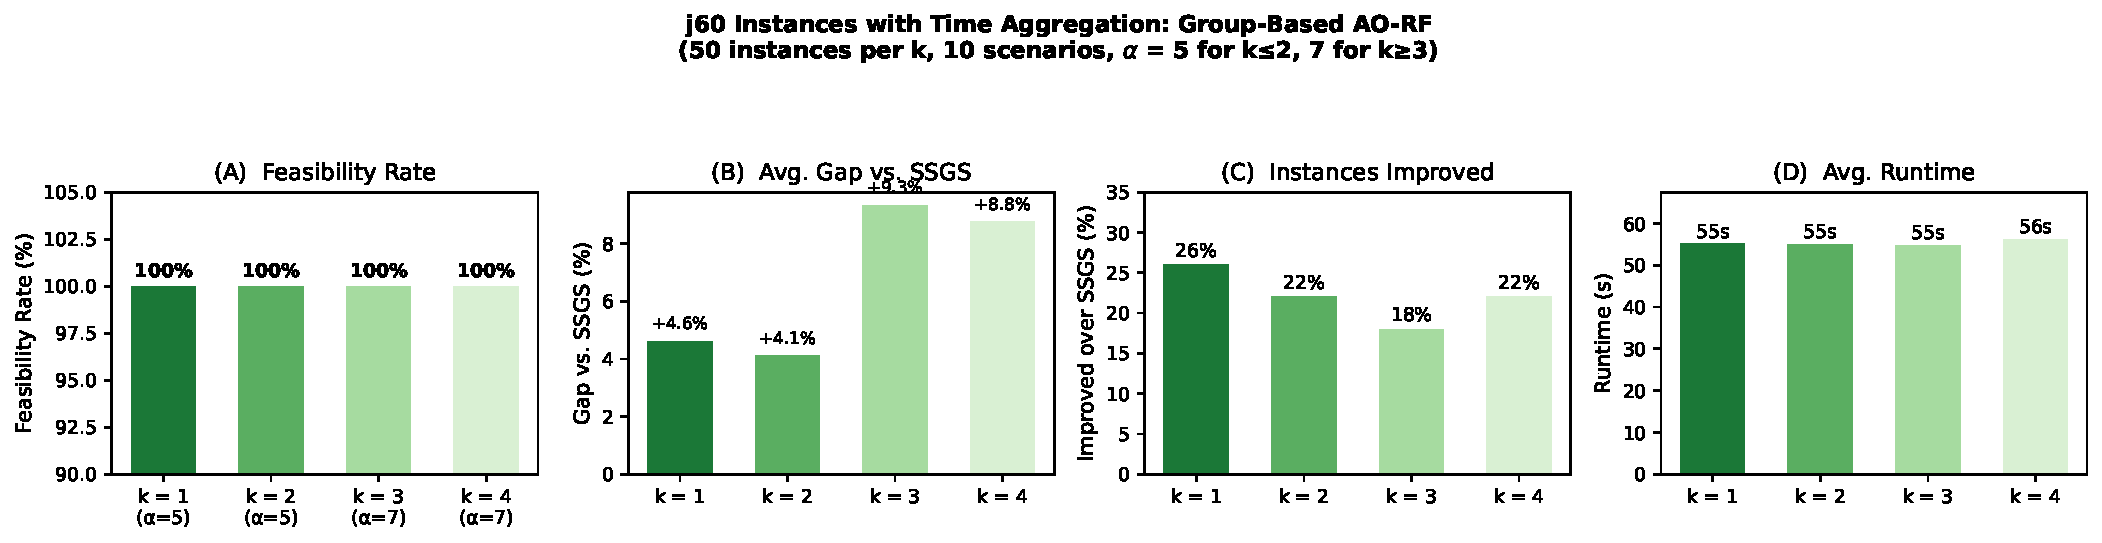
\includegraphics[width=\textwidth]{exp5_j60_figure}
  \caption{Group-based R\&F with time aggregation on j60
           instances ($|S|=10$, 50 instances per~$|K|$,
           $\alpha=5$ for $|K|\leq 2$, $\alpha=7$ for
           $|K|\geq 3$).
           \textbf{(A)}~Feasibility rate.
           \textbf{(B)}~Mean makespan gap relative to the
           SSGS warm-start.
           \textbf{(C)}~Number of instances with makespan
           strictly below the SSGS warm-start.
           \textbf{(D)}~Mean wall-clock runtime.}
  \label{fig:j60_results}
\end{figure}
% ============================================================
\section{Ablation Study: Feature Selection for Activity Clustering}
\label{sec:ablation}
% ============================================================
The group-based AO-RF relies on Ward hierarchical clustering
applied to a feature matrix extracted from the instance data
(Chapter~\ref{chap:grouprf}, Section~\ref{sec:features}). The
\texttt{EnrichedFeatureExtractor} computes a comprehensive
candidate pool of $18 + 8|K|$ features ($50$ for $|K|=4$),
organised into seven conceptual groups spanning network position
(Groups~A--B, $7$~features), duration (Group~C, $3$~features),
urgency (Group~D, $3$~features), timing (Group~E,
$4$~features), and stochastic resource load (Groups~F--G,
$1 + 8|K|$~features). Not all features necessarily contribute
to clustering quality: including irrelevant or redundant
dimensions can inflate the Ward distance metric and cause the
clusterer to merge activities that share peripheral statistics
but have incompatible scheduling structures. A systematic
ablation over the full candidate pool is therefore required to
determine which features, and which combinations, yield the
best trade-off between feasibility, solution quality, and
runtime.
The ablation is conducted on 10 PSPLIB j60 instances with
$|K|=4$ resource types and time aggregation $\alpha = 7$. For
analysis purposes the seven conceptual groups are decomposed
into 14 semantically defined sub-groups (e.g.\ Group~G is split
into eight per-statistic sub-groups \texttt{res\_mean},
\texttt{res\_cv}, etc.), enabling fine-grained isolation of each
feature dimension's contribution.
% ------------------------------------------------------------
\subsection{Study Design}
\label{subsec:ablation_design}
% ------------------------------------------------------------
The 50 candidate features span 14 semantically defined groups:
\begin{table}[htbp]
\centering
\renewcommand{\arraystretch}{1.30}
\caption{Feature sub-groups in the ablation study ($|K|=4$).
         Groups marked $^{\dagger}$ are per-resource
         ($|K|$~features each).}
\label{tab:ablation_feature_groups}
\begin{tabular}{l l r l}
\hline
\textbf{ID} & \textbf{Group} & $p$ & \textbf{Features} \\
\hline
A & \texttt{net\_basic} (net4)   & 4 & prec.\ level, in/out-degree, longest path \\
B & \texttt{net\_ext}            & 3 & transitive succ./pred., betweenness \\
C & \texttt{duration}            & 3 & duration, rel.\ duration, duration rank \\
D & \texttt{urgency}             & 3 & slack, pressure index, $n_{\text{concurrent}}$ \\
E & \texttt{timing}              & 4 & rel.\ ES/LS, critical path, float ratio \\
F & \texttt{res\_joint}          & 1 & resource pressure \\
G$^{\dagger}$ & \texttt{res\_mean}  & 4 & $\overline{W}_k$ \\
H$^{\dagger}$ & \texttt{res\_cv}    & 4 & $\mathrm{CV}(W_k)$ \\
I$^{\dagger}$ & \texttt{res\_iqr}   & 4 & $\mathrm{IQR}(W_k)$ \\
J$^{\dagger}$ & \texttt{res\_tail}  & 4 & tail ratio$(W_k)$ \\
K$^{\dagger}$ & \texttt{res\_max}   & 4 & $\max(W_k)$ \\
L$^{\dagger}$ & \texttt{res\_min}   & 4 & $\min(W_k)$ \\
M$^{\dagger}$ & \texttt{res\_range} & 4 & range$(W_k)$ \\
N$^{\dagger}$ & \texttt{res\_pnz}   & 4 & $P(\text{nonzero},W_k)$ \\
\hline
 & \textbf{Total}              & \textbf{50} & \\
\hline
\end{tabular}
\end{table}
\noindent
The experiment proceeds in three phases:
\begin{enumerate}
  \item \textbf{Phase~1 (single-group baselines):}
        Each of the 14 groups is used alone for clustering
        ($14$ configurations).
  \item \textbf{Phase~2 (net4 augmented):}
        The four-feature net4 baseline is combined with each
        of the remaining 13 groups
        ($13$ configurations).
  \item \textbf{Phase~3 (aggregate controls):}
        Four larger unions are tested:
        all network (A\,+\,B, $p{=}7$),
        all structural (A--F, $p{=}18$),
        all resource (F--N, $p{=}33$),
        and the full 50-feature set ($p{=}50$).
\end{enumerate}
\noindent
All runs use $|S|=10$ scenarios,
$T_{\max}=600\,\text{s}$,
$T_{\mathrm{model}}=60\,\text{s}$,
$\theta_{\mathrm{merge}}=2.5$,
$\theta_{\mathrm{corr}}=0.95$,
\texttt{stop\_on\_first\_feasible\,=\,True},
and \texttt{max\_no\_improve\,=\,0}.
% ------------------------------------------------------------
\subsection{Results}
\label{subsec:ablation_results}
% ------------------------------------------------------------
Table~\ref{tab:comp_ablation} reports the key metrics for
all 32 configurations. The net4 configuration (Group~A alone)
serves as the reference baseline.
\begin{table}[htbp]
\centering
\renewcommand{\arraystretch}{1.25}
\caption{Ablation study results: j60, $|K|=4$,
         $\alpha=7$, 10 instances.
         \emph{Feas.}: feasible instances;
         $\bar{\delta}$: mean gap vs.\ SSGS~(\%);
         $\bar{t}$: mean runtime~(s).
         Bold marks best gap at full feasibility.}
\label{tab:comp_ablation}
\begin{tabular}{l r r r r}
\hline
\textbf{Config} & $p$ &
\textbf{Feas.} &
$\bar{\delta}$ (\%) &
$\bar{t}$ (s) \\
\hline
\multicolumn{5}{l}{\emph{Reference}} \\
\textbf{net4}                & 4  & \textbf{10} & \textbf{8.09} & 72.3 \\
\hline
\multicolumn{5}{l}{\emph{Phase~1: single group alone}} \\
\texttt{net\_basic}          & 4  & 10 & 8.09 & 60.2 \\
\texttt{net\_ext}            & 3  & 10 & 8.09 & 72.4 \\
\texttt{duration}            & 3  & 10 & 8.09 & 60.3 \\
\texttt{urgency}             & 3  &  9 & 8.76 & 66.3 \\
\texttt{timing}              & 4  & 10 & 8.09 & 60.2 \\
\texttt{res\_joint}          & 1  & 10 & 8.09 & 72.3 \\
\texttt{res\_mean}           & 4  & 10 & 8.09 & 56.1 \\
\texttt{res\_cv}             & 4  &  9 & 7.72 & 110.9 \\
\texttt{res\_iqr}            & 4  & 10 & 8.09 & 52.3 \\
\texttt{res\_tail}           & 4  &  9 & 7.72 & 103.8 \\
\texttt{res\_max}            & 4  & 10 & 8.09 & 57.1 \\
\texttt{res\_min}            & 4  & 10 & 8.09 & 57.6 \\
\texttt{res\_range}          & 4  & 10 & 8.09 & 56.4 \\
\texttt{res\_pnz}            & 4  &  8 & 8.43 & 152.1 \\
\hline
\multicolumn{5}{l}{\emph{Phase~2: net4 + one group}} \\
\texttt{+net\_ext}           & 7  & 10 & 8.09 & 72.4 \\
\texttt{+duration}           & 7  & 10 & 8.09 & 60.2 \\
\texttt{+urgency}            & 7  & 10 & 8.09 & 55.9 \\
\texttt{+timing}             & 8  & 10 & 8.09 & 60.4 \\
\texttt{+res\_joint}         & 5  & 10 & 8.09 & 60.4 \\
\texttt{+res\_mean}          & 8  & 10 & 8.09 & 60.3 \\
\texttt{+res\_cv}            & 8  &  8 & 8.43 & 153.8 \\
\texttt{+res\_iqr}           & 8  &  9 & 7.72 & 104.3 \\
\texttt{+res\_tail}          & 8  &  7 & 9.63 & 207.2 \\
\texttt{+res\_max}           & 8  &  9 & 7.82 & 107.7 \\
\texttt{+res\_min}           & 8  & 10 & 8.09 & 56.0 \\
\texttt{+res\_range}         & 8  &  9 & 7.82 & 105.1 \\
\texttt{+res\_pnz}           & 8  &  9 & 8.76 & 94.6 \\
\hline
\multicolumn{5}{l}{\emph{Phase~3: aggregate controls}} \\
\texttt{all\_net}            & 7  & 10 & 8.09 & 66.3 \\
\texttt{all\_struct}         & 18 &  9 & 8.18 & 98.5 \\
\texttt{all\_res}            & 33 &  9 & 8.76 & 99.2 \\
\texttt{all\_50}             & 50 & 10 & 8.09 & 53.6 \\
\hline
\end{tabular}
\end{table}
% ------------------------------------------------------------
\subsection{Analysis}
\label{subsec:ablation_analysis}
% ------------------------------------------------------------
Three findings emerge from the ablation:
\textbf{No configuration improves on net4 in both gap and
feasibility.}
Among the 31 alternative configurations, only
\texttt{res\_cv} and \texttt{res\_tail} (Phase~1) and
\texttt{net4+res\_iqr} (Phase~2) achieve a lower mean gap
($7.72\%$ vs.\ $8.09\%$), but each loses at least one
feasible instance (9/10) and incurs substantially higher
runtime ($103$--$154\,\text{s}$ vs.\ $72\,\text{s}$).
In a scheduling context where feasibility is the primary
concern, these trade-offs are unfavourable.
\textbf{Adding features to net4 can \emph{hurt} performance.}
Several Phase~2 combinations degrade both feasibility and
runtime: \texttt{net4+res\_tail} drops to only 7/10 feasible
instances with a mean runtime of $207\,\text{s}$, and
\texttt{net4+res\_cv} drops to 8/10 feasible at $154\,\text{s}$.
The additional feature dimensions introduce noise into the
Ward distance metric, causing the clusterer to merge
activities that share resource statistics but have
incompatible precedence structures.
\textbf{The full 50-feature set recovers but does not improve.}
The all\_50 configuration ($p=50$) matches net4 exactly
in both gap ($8.09\%$) and feasibility (10/10), demonstrating
that correlation-based pruning ($\theta_{\mathrm{corr}}=0.95$)
successfully removes redundant features. However, the
12.5$\times$ increase in feature dimensionality provides no
benefit, confirming that the informative signal resides
entirely in the four network features.
% ------------------------------------------------------------
\subsection{Default Feature Subset}
\label{subsec:ablation_default}
% ------------------------------------------------------------
Across 50 candidate features and 32 configurations, the
four-feature network subset (Group~A) is Pareto-optimal: no
configuration achieves both a lower gap and equal or higher
feasibility. The default feature subset is therefore:
\begin{equation}
  \mathcal{F}_{\text{default}}
  = \{\texttt{precedence\_level},\;
      \texttt{in\_degree},\;
      \texttt{out\_degree},\;
      \texttt{longest\_path\_to\_sink}\}.
  \label{eq:default_features_exp}
\end{equation}
This result, obtained on the largest instance class (j60) with
time aggregation, provides strong empirical support for the
default adopted in Section~\ref{subsec:default_features}. All
preceding and subsequent experiments in this thesis use
$\mathcal{F}_{\text{default}}$ for activity clustering.
% ============================================================
\section{Sensitivity Analysis: Time Aggregation Factor $\alpha$}
\label{sec:alpha_sensitivity}
% ============================================================
The time aggregation extension introduced in
Chapter~\ref{chap:grouprf} compresses the time horizon from
$|T|$ to $\lceil |T| / \alpha \rceil$ periods, reducing the
number of variables and constraints per subproblem. The choice
of~$\alpha$ controls the trade-off between model fidelity and
computational tractability: a small~$\alpha$ preserves temporal
resolution but results in larger subproblems, while a
large~$\alpha$ sharply reduces model size at the cost of
coarser scheduling granularity and potentially degraded solution
quality. This section investigates this trade-off systematically
across instance sizes j30, j60, and j120, with
$|K| \in \{1, 2, 3, 4\}$ resource types and $|S| = 10$
scenarios.
% ------------------------------------------------------------
\subsection{Experimental Design}
\label{subsec:alpha_design}
% ------------------------------------------------------------
For each combination of instance size and resource count, the
group-based R\&F heuristic was executed on 10 instances with
varying~$\alpha$ values. The tested values were selected to span
a wide range of compression ratios:
\begin{itemize}
  \item \textbf{j30} ($|K| \in \{3, 4\}$):
        $\alpha \in \{1, 2, 3, 5, 7\}$, where $\alpha = 1$
        corresponds to no aggregation.
  \item \textbf{j60} ($|K| \in \{1, 2, 3, 4\}$):
        $\alpha \in \{3, 5, 7, 10, 13\}$.
  \item \textbf{j120} ($|K| \in \{1, 2, 3, 4\}$):
        $\alpha \in \{7, 10, 13, 15, 20\}$.
\end{itemize}
\noindent
A per-subproblem time limit of $T_{\mathrm{model}} = 60$\,s and
a total wall-clock limit of $T_{\max} = 600$\,s were used for
all runs.
% ------------------------------------------------------------
\subsection{Results}
\label{subsec:alpha_results}
% ------------------------------------------------------------
Table~\ref{tab:alpha_optimal} reports, for each instance size
and resource count, the smallest~$\alpha$ that achieves 100\%
feasibility together with the corresponding mean gap relative
to the SSGS warm-start and mean runtime.
\begin{table}[htbp]
\centering
\renewcommand{\arraystretch}{1.35}
\caption{Optimal time aggregation factor~$\alpha^*$: smallest
         $\alpha$ achieving 100\% feasibility (10 instances each).
         $\bar{\delta}$: mean gap vs.\ SSGS~(\%);
         $\bar{t}$: mean runtime~(s). The j120/$|K|{=}2$ entry
         marks the best available ($\alpha{=}15$, 90\% feasibility).}
\label{tab:alpha_optimal}
\begin{tabular}{l r r r r}
\hline
\textbf{Size / $|K|$} &
$\alpha^*$ &
\textbf{Feas.~(\%)} &
$\bar{\delta}$ (\%) &
$\bar{t}$ (s) \\
\hline
j30 / 3  &  2 & 100 & $-$0.16 & 58.5 \\
j30 / 4  &  2 & 100 & $-$0.09 & 72.4 \\
\hline
j60 / 1  &  5 & 100 &    5.81 & 53.2 \\
j60 / 2  &  7 & 100 &   15.38 & 53.2 \\
j60 / 3  &  7 & 100 &   14.53 & 51.5 \\
j60 / 4  &  7 & 100 &    8.09 & 57.0 \\
\hline
j120 / 1 & 13 & 100 &   41.26 & 53.0 \\
j120 / 2 & 15 &  90 &   42.65 & 88.3 \\
j120 / 3 & 20 & 100 &   77.63 & 40.4 \\
j120 / 4 & 15 & 100 &   37.73 & 50.4 \\
\hline
\end{tabular}
\end{table}
Table~\ref{tab:alpha_tradeoff} provides a detailed view of the
feasibility--quality trade-off across all tested $\alpha$ values
for j60 instances.
\begin{table}[htbp]
\centering
\renewcommand{\arraystretch}{1.35}
\caption{Time aggregation sensitivity for j60 instances
         (10 instances per cell).
         \emph{Feas.}: feasible count of 10;
         $\bar{\delta}$: mean gap vs.\ SSGS~(\%).}
\label{tab:alpha_tradeoff}
\begin{tabular}{r r r r r r r r r}
\hline
& \multicolumn{2}{c}{$|K|=1$}
& \multicolumn{2}{c}{$|K|=2$}
& \multicolumn{2}{c}{$|K|=3$}
& \multicolumn{2}{c}{$|K|=4$} \\
\cmidrule(lr){2-3} \cmidrule(lr){4-5}
\cmidrule(lr){6-7} \cmidrule(lr){8-9}
$\alpha$ & Feas. & $\bar{\delta}$
         & Feas. & $\bar{\delta}$
         & Feas. & $\bar{\delta}$
         & Feas. & $\bar{\delta}$ \\
\hline
 3 &  5 &  0.3 &  0 &  1.8 &  0 &  0.6 &  0 &  0.9 \\
 5 & 10 &  5.8 &  9 &  7.1 &  5 &  8.5 &  7 &  6.8 \\
 7 & 10 & 12.8 & 10 & 15.4 & 10 & 14.5 & 10 &  8.1 \\
10 & 10 & 32.5 & 10 & 32.4 & 10 & 30.5 & 10 & 29.4 \\
13 &  --- & --- & --- & --- & 10 & 43.3 & 10 & 39.3 \\
\hline
\end{tabular}
\end{table}
Figure~\ref{fig:alpha_sensitivity} visualises the full
trade-off across all three instance sizes. The left column
confirms that feasibility jumps from $0\%$ to $100\%$ once
$\alpha$ passes a size- and $|K|$-dependent threshold. The
centre column shows the corresponding cost in solution quality,
and the right column illustrates the runtime reduction that
accompanies higher aggregation.
\begin{figure}[htbp]
  \centering
  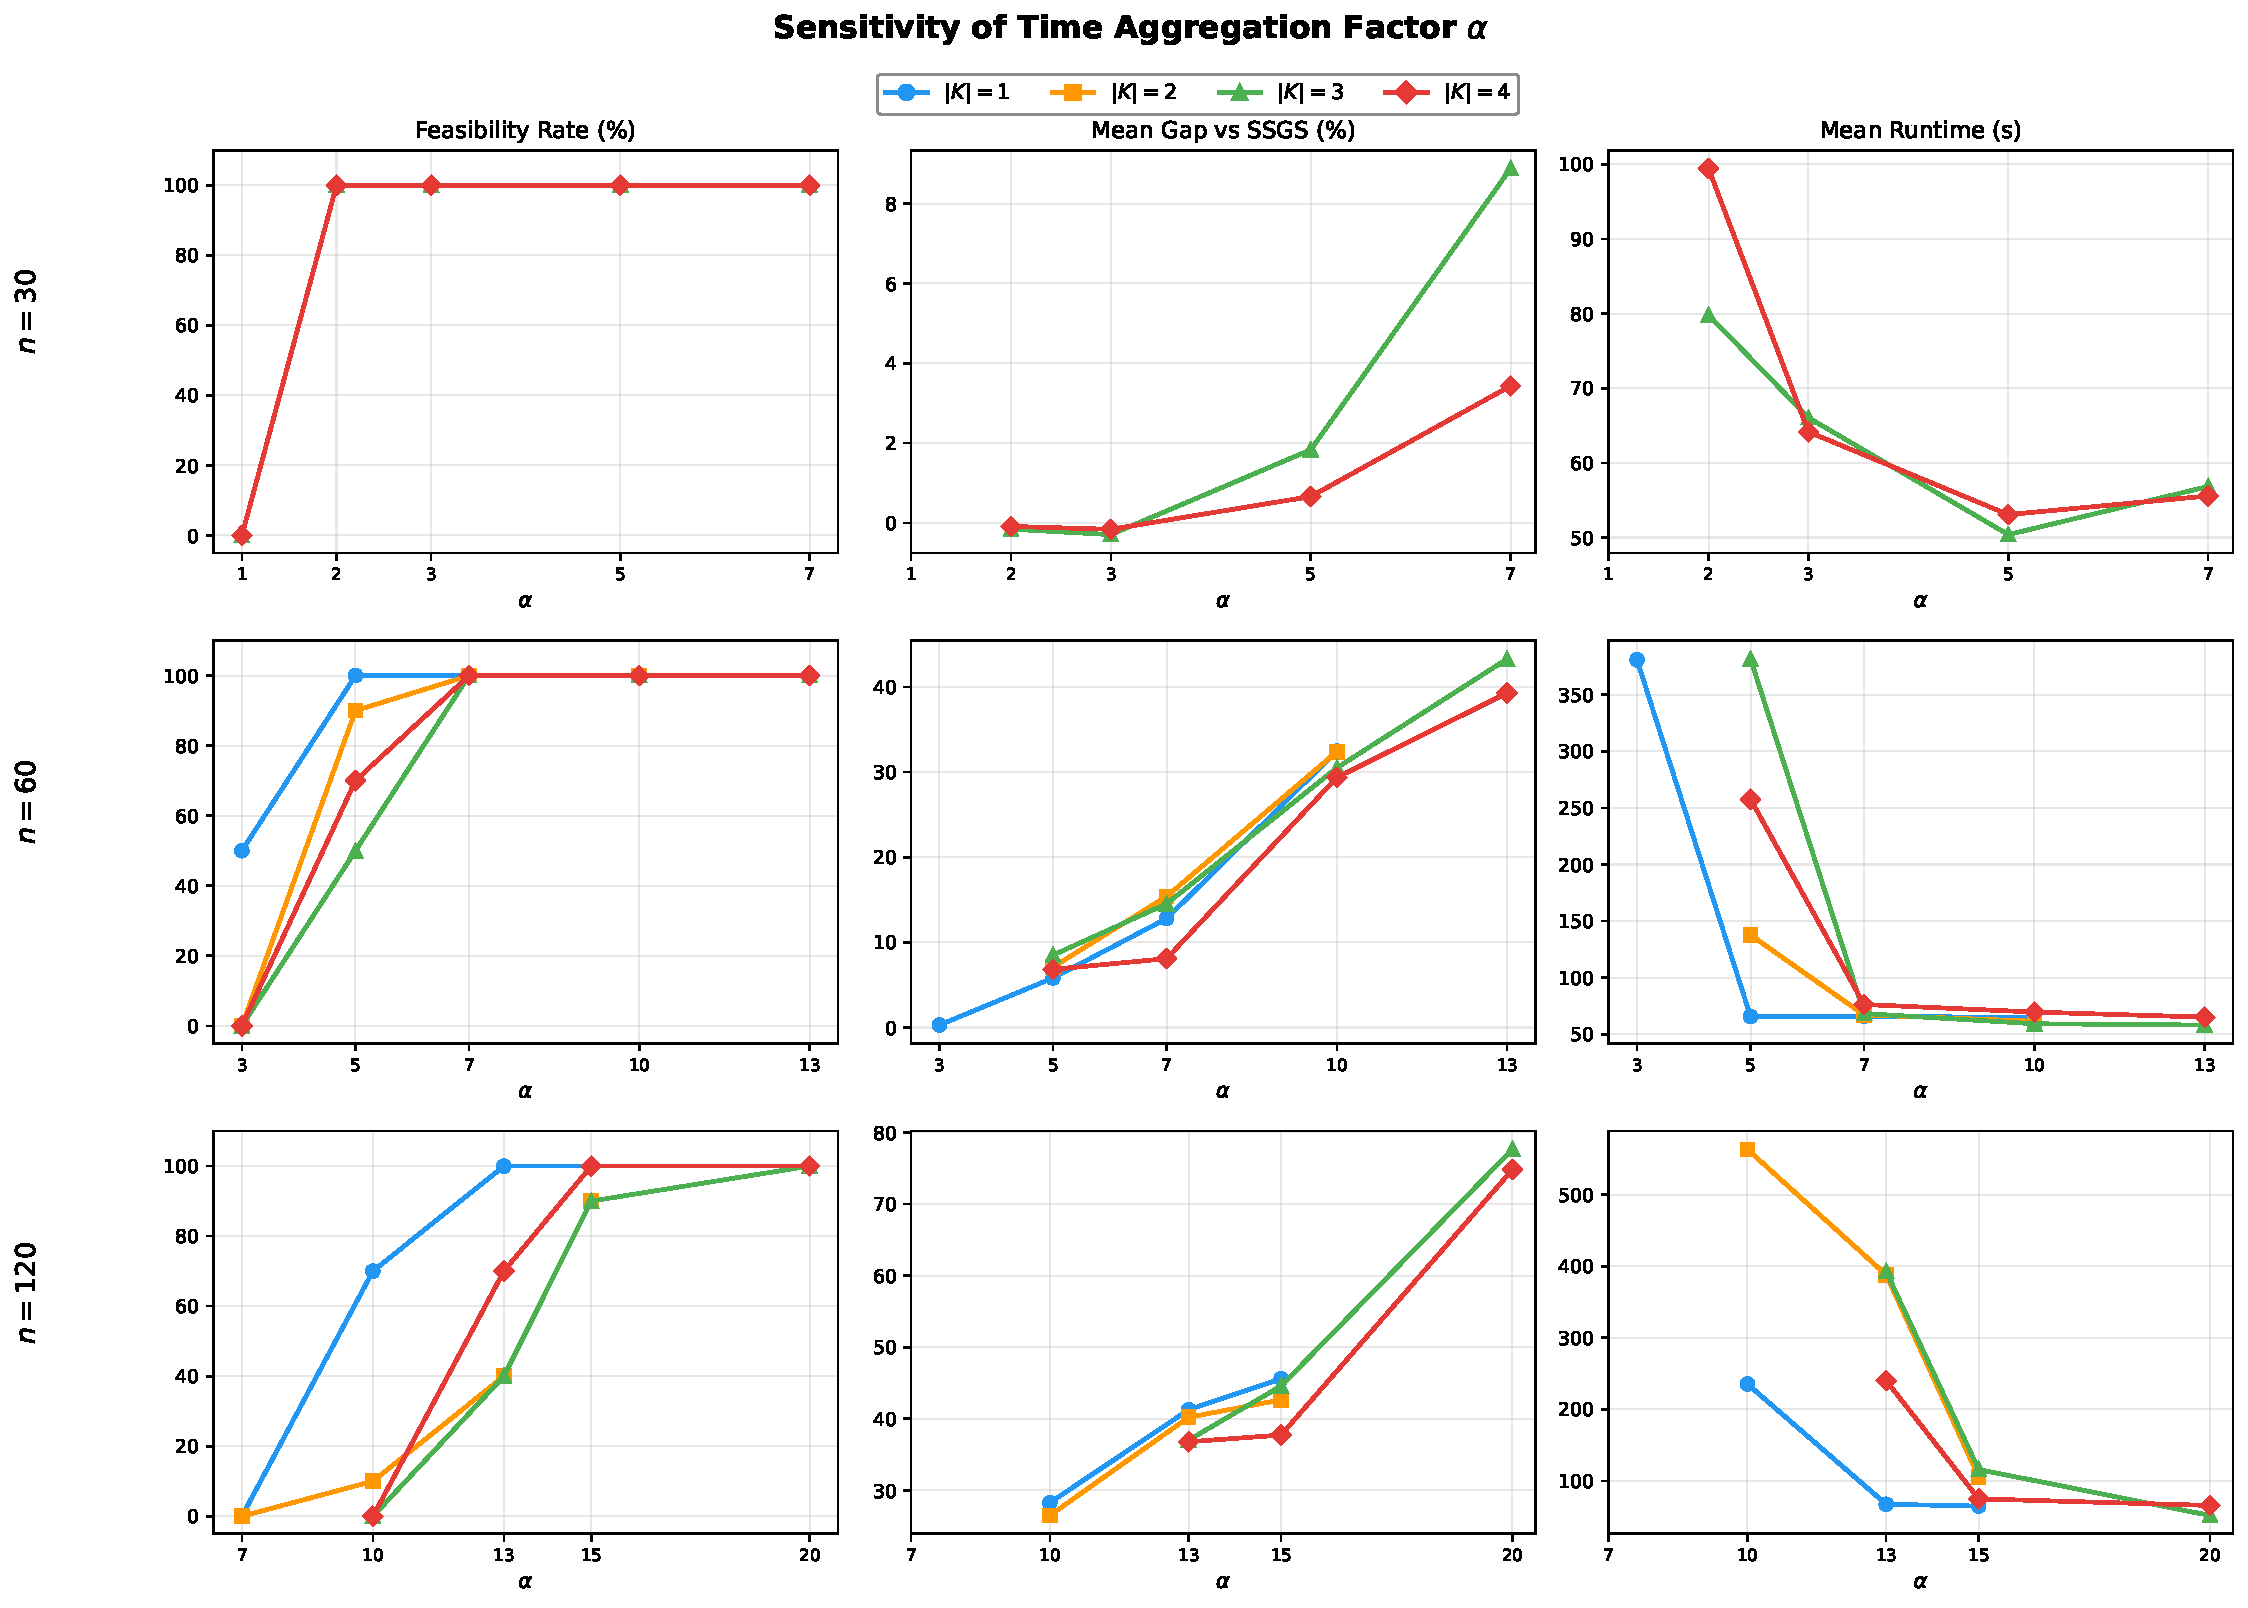
\includegraphics[width=\textwidth]{alpha_sensitivity_figure}
  \caption{Sensitivity of the time aggregation factor~$\alpha$
           across j30, j60, and j120 instances
           ($|S|=10$, 10 instances per configuration).
           \textbf{Left:} Feasibility rate~(\%).
           \textbf{Centre:} Mean makespan gap relative to the
           SSGS warm-start~(\%); points with $0\%$ feasibility
           are omitted.
           \textbf{Right:} Mean wall-clock runtime~(s).
           Each line represents one resource count~$|K|$.}
  \label{fig:alpha_sensitivity}
\end{figure}
\subsection{Discussion}
\label{subsec:alpha_discussion}
Three observations emerge from the sensitivity analysis.
\paragraph{Feasibility requires sufficient aggregation.}
The left column of Figure~\ref{fig:alpha_sensitivity} shows that
without time aggregation ($\alpha = 1$), the j30 model with
$|K| = 4$ contains over 300\,000 variables
(cf.\ Table~\ref{tab:model_size}), and no instance is solved
to feasibility within the 600\,s budget. Even moderate
aggregation ($\alpha = 2$) reduces the effective time horizon
by half and immediately achieves 100\% feasibility on j30. The
pattern repeats at larger scales: for j60, $\alpha \geq 5$ is
needed at $|K| = 1$, while $\alpha \geq 7$ is required for
$|K| \geq 2$. For j120, the threshold rises to
$\alpha \geq 13$--$20$, reflecting the much larger model
dimensions. In each row of the figure, the feasibility curves
show a sharp transition from $0\%$ to $90$--$100\%$ once
$\alpha$ crosses the critical value.
\paragraph{Quality degrades gracefully.}
The centre column of Figure~\ref{fig:alpha_sensitivity} shows
that the gap rises monotonically with~$\alpha$ in all
configurations, confirming the expected trade-off between model
fidelity and tractability. On j30, the optimal $\alpha^* = 2$
achieves a \emph{negative} mean gap ($-0.16\%$ for $|K| = 3$,
$-0.09\%$ for $|K| = 4$), meaning the MIP solver actually
improves upon the SSGS warm-start at this compression level.
On j60, the gap at the optimal~$\alpha^*$ ranges from $5.8\%$
($|K|=1$) to $15.4\%$ ($|K|=2$). On j120, the gap is
necessarily larger (38--78\%) because of the aggressive
compression required for tractability.
\paragraph{Runtime drops sharply with aggregation.}
The right column of Figure~\ref{fig:alpha_sensitivity} shows
that runtime falls steeply once $\alpha$ passes the feasibility
threshold. On j60, for instance, $|K|=1$ at $\alpha=3$ averages
$381$\,s (with only $50\%$ feasibility), but by $\alpha=5$ all
instances are feasible in $66$\,s. Beyond the threshold the
curves flatten, as the per-subproblem time limit rather than the
model size becomes the binding constraint.
\paragraph{Resource count affects the optimal $\alpha$.}
For j60, $|K| = 1$ achieves feasibility at $\alpha = 5$, while
$|K| \geq 2$ requires $\alpha = 7$. Additional resource types
introduce more $r_{ikt\pi}$ variables per time period, making
the subproblems harder to solve within the per-subproblem time
limit. Higher aggregation compensates by reducing the number of
time periods. The same pattern is visible for j120 in
Figure~\ref{fig:alpha_sensitivity}, where $|K|=2$ lags behind
$|K|=1$ by roughly one step in~$\alpha$.
% ============================================================
\section{Scenario Reduction Experiment (j120, $|K|=4$)}
\label{sec:scen_red_exp}
% ============================================================
Per-group scenario reduction
(Section~\ref{subsec:scen_red}) reduces the number of
stochastic scenarios in each group subproblem from $|S|$ to
$n_{\mathrm{keep}}$, with the goal of making larger instances
tractable. This section evaluates the reduction strategies on
j120 instances, where the full $|S|=10$ model is prohibitively
large without reduction.
\subsection{Experimental Design}
The experiment compares six configurations on 10 j120 instances
with $|K|=4$, $\alpha=15$, $T_{\max}=600\,\text{s}$, and
$T_{\mathrm{model}}=60\,\text{s}$:
\begin{itemize}
  \item \textbf{Baseline}: full $|S|=10$ scenarios, no reduction.
  \item \textbf{Global naive}: keep the first $n_{\mathrm{keep}}=3$
        scenarios (trivial baseline).
  \item \textbf{Global random}: randomly sample 3 scenarios.
  \item \textbf{Global K-medoids}: PAM K-medoids on the full
        instance workload vectors, select 3 representative
        scenarios globally.
  \item \textbf{Global backward}: Heitsch--R\"omisch backward
        deletion \parencite{Heitsch2003}, retain 3 scenarios.
  \item \textbf{Per-group K-medoids}: PAM K-medoids applied
        separately to each group's workload vectors; each group
        selects its own 3 representative scenarios from the full
        $|S|=10$ set.
\end{itemize}
\noindent
The four global methods reduce the instance to 3 scenarios
\emph{before} the R\&F loop, so every group subproblem uses the
same reduced set. The per-group method retains all 10 scenarios
in the instance data but rebuilds each group's subproblem MIP on
only 3 group-specific medoids.
\subsection{Results}
Table~\ref{tab:scen_red_j120} reports the aggregate results.
\begin{table}[htbp]
\centering
\renewcommand{\arraystretch}{1.35}
\caption{Scenario reduction results: j120, $|K|=4$,
         $\alpha=15$, 10 instances.
         \emph{Feas.}: feasible instances;
         $\bar{\delta}$: mean gap vs.\ SSGS~(\%);
         $\bar{t}$: mean runtime~(s).}
\label{tab:scen_red_j120}
\begin{tabular}{l r r r r}
\hline
\textbf{Method} & $|S_{\text{used}}|$ &
\textbf{Feas.} &
$\bar{\delta}$ (\%) &
$\bar{t}$ (s) \\
\hline
Baseline (no reduction)       & 10 & 10 & 37.73 &  79.0 \\
\hline
Global naive                  &  3 & 10 & 33.27 &  43.5 \\
Global random                 &  3 & 10 & 32.85 &  43.2 \\
Global K-medoids              &  3 & 10 & 31.83 &  43.5 \\
Global backward               &  3 & 10 & 32.01 &  43.0 \\
\hline
Per-group K-medoids           & 10 & 10 & \textbf{10.30} & 103.4 \\
\hline
\end{tabular}
\end{table}
\subsubsection*{Global Reduction}
All four global methods achieve 100\% feasibility and reduce
runtime by approximately $45\%$ (from 79\,s to 43\,s) by
cutting the scenario dimension from 10 to 3. Solution quality
also improves slightly (gaps of 31--33\% vs.\ 37.73\%), because
the smaller model is easier for the solver to explore within the
time limit. Among the global methods, PAM K-medoids achieves
the best gap (31.83\%), followed by backward deletion (32.01\%),
confirming that principled scenario selection outperforms naive
or random approaches, though the differences are modest.
\subsubsection*{Per-Group Reduction}
The per-group K-medoids method achieves dramatically better
solution quality: a mean gap of $10.30\%$, a $3.6\times$
improvement over the best global method. This comes at the cost
of higher runtime ($103\,\text{s}$ vs.\ $43\,\text{s}$), because
the per-group method retains all 10 scenarios in the instance
data and performs a fresh K-medoids selection for each group
subproblem. However, the runtime is still well within the
$T_{\max}=600\,\text{s}$ budget.
The advantage of per-group reduction is that each group's
subproblem uses the 3 scenarios most informative for \emph{that
group's} activities. A group dominated by resource~$k=1$
variation selects different representative scenarios than a
group dominated by resource~$k=3$ variation, whereas a global
reduction must compromise across all activities.
\subsection{Scalability to j120 Across All $|K|$}
To assess whether per-group reduction scales across
resource-flexibility levels, the experiment was extended to
$|K| \in \{1, 2, 3, 4\}$ on 50 j120 instances each.
Table~\ref{tab:scen_red_j120_allk} reports the results.
\begin{table}[htbp]
\centering
\renewcommand{\arraystretch}{1.35}
\caption{Per-group K-medoids scenario reduction on j120 instances,
         $|K|=1$--$4$, 50 instances each.
         \emph{Feas.}: feasible instances;
         $\bar{\delta}$: mean gap vs.\ SSGS~(\%).}
\label{tab:scen_red_j120_allk}
\begin{tabular}{l r r r r r r r}
\hline
 & \multicolumn{3}{c}{\textbf{Baseline}} &
   \multicolumn{3}{c}{\textbf{Per-group K-med.}} \\
\cline{2-4} \cline{5-7}
$|K|$ &
\textbf{Feas.} & $\bar{\delta}$ (\%) & $\bar{t}$ (s) &
\textbf{Feas.} & $\bar{\delta}$ (\%) & $\bar{t}$ (s) \\
\hline
1 & 50 & 15.73 &  63.9 & 49 & $-$12.94 & 116.5 \\
2 & 49 & 22.66 &  63.9 & 49 & $-$13.18 & 122.5 \\
3 & 41 & 18.63 &  94.5 & 46 & $-$13.74 & 125.4 \\
4 & 46 & 16.24 &  92.2 & 48 & $-$16.70 & 127.0 \\
\hline
\end{tabular}
\end{table}
The per-group K-medoids method consistently achieves
\emph{negative} mean gaps, meaning it improves upon the SSGS
warm-start on average. This is in stark contrast to the
baseline, which has positive gaps of $16$--$23\%$ across all
$|K|$ values. The feasibility advantage is most pronounced at
$|K|=3$ ($92\%$ vs.\ $82\%$, $+10$ pp) and $|K|=4$ ($96\%$
vs.\ $92\%$, $+4$ pp). Runtime is approximately $1.4\times$
higher than the baseline due to the per-group medoid computation,
but remains well within practical limits.
These results demonstrate that per-group scenario reduction is
essential for scaling the group-based R\&F to j120 instances:
global reduction saves runtime but provides little quality
improvement, while per-group reduction exploits the
group-local structure of the decomposition to select maximally
informative scenarios for each subproblem.
% ============================================================
\section{Discussion}
\label{sec:discussion}
% ============================================================
\subsection{When Does Grouping Help?}
\label{subsec:when_grouping}
Across all four instance sizes, the group-based decomposition
produces faster runtimes and, in most configurations, at least
as many feasible solutions as the baseline.
For j10 (Figure~\ref{fig:j10_comparison}), Ward clustering
collapses all activities into a single group
($\bar{m} = 1$), so the R\&F effectively becomes a
one-shot MIP solve with a warm start. This yields speedups of
$3$--$6\times$ at $|K| \in \{1,2\}$ and $12\times$ at $|K|=4$,
though at $|K|=3$ a single outlier instance inflates the
group-based mean runtime, making the median ($1.8\times$ faster)
the fairer comparison. The group-based method recovers
feasibility on 7 instances the baseline misses at $|K|=4$
($p = 0.016$, McNemar test). Solution quality is the same in
over $97\%$ of jointly feasible cases.
For j30 without time aggregation
(Figure~\ref{fig:j30_comparison}), the speedup is larger,
reaching $4$--$5\times$, because the baseline wastes time cycling
through 16--28 single-activity subproblems while the
group-based method finishes in 2--3 iterations. Feasibility is
also higher at $|K| \leq 3$ (up to $+8$ percentage points at
$|K|=1$). Adding time aggregation with $\alpha = 2$
(Figure~\ref{fig:j30_alpha2}) pushes feasibility to $100\%$ at
$|K| \leq 2$ and $92$--$98\%$ at $|K| \geq 3$, and the mean
gap turns negative at every resource-flexibility level, meaning
the MIP solver improves on the SSGS heuristic on average.
For j60 (Figure~\ref{fig:j60_results}), the model without time
aggregation is simply too large for either method. With
$\alpha \in \{5, 7\}$, the group-based approach solves all 200
instances to feasibility, though the mean gap of $4$--$9\%$
relative to the SSGS warm-start reflects the coarsening inherent
in the time aggregation. Even so, $22\%$ of instances end up
with a strictly better makespan than the heuristic. The
sensitivity analysis (Figure~\ref{fig:alpha_sensitivity}) shows
how the feasibility--quality trade-off varies with~$\alpha$
across all four instance sizes.
For j120 (Table~\ref{tab:scen_red_j120_allk}), per-group
scenario reduction proves essential. The baseline with $\alpha=15$
achieves 82--100\% feasibility but mean gaps of 16--23\%.
Per-group K-medoids reduction pushes the mean gap to
\emph{negative} values ($-13\%$ to $-17\%$), meaning the MIP
consistently improves upon the SSGS warm-start. Feasibility also
rises at higher $|K|$ ($+10$~pp at $|K|=3$, $+4$~pp at $|K|=4$).
This demonstrates that the group-based pipeline, equipped with
both time aggregation and per-group scenario reduction, scales
to the largest PSPLIB instances while maintaining solution quality
that surpasses the heuristic warm-start.
\subsection{Statistical Validation}
\label{subsec:stat_tests}
The aggregate comparisons in the preceding sections suggest that
the group-based R\&F is faster and at least as reliable as the
baseline, but aggregate means can be misleading. To test whether
the observed differences are statistically significant, we apply
a Wilcoxon signed-rank test to the paired runtime observations
(one pair per instance, restricted to jointly feasible instances)
and a McNemar exact test to the paired feasibility outcomes
(feasible vs.\ not feasible under each method). Both tests are
non-parametric and do not assume normality, which is appropriate
given the skewed runtime distributions typical of MIP solvers.
Table~\ref{tab:stat_tests} reports the results.
\begin{table}[htbp]
\centering
\renewcommand{\arraystretch}{1.35}
\caption{Statistical tests: baseline vs.\ group-based R\&F.
         \emph{JF}: jointly feasible instances;
         $\bar{t}_B$, $\bar{t}_G$: mean runtime~(s);
         \emph{W-RT}: Wilcoxon signed-rank $p$-value on
         paired runtimes;
         \emph{McN}: McNemar exact $p$-value on feasibility.
         Significant results ($p < 0.05$) are marked
         with~$^{*}$.}
\label{tab:stat_tests}
\begin{tabular}{l r r r r r l l}
\hline
\textbf{Size / $|K|$} &
\textbf{JF} &
$\bar{t}_B$ &
$\bar{t}_G$ &
\textbf{Speedup} &
\textbf{W-RT} &
\textbf{McN} \\
\hline
j10 / 1 & 50 & 112.5 &  33.4 & $3.4\times$ & ${<}\,0.001^{*}$ & 1.000 \\
j10 / 2 & 50 & 176.4 &  28.8 & $6.1\times$ & ${<}\,0.001^{*}$ & 1.000 \\
j10 / 3 & 50 & 137.6 & 298.5 & $0.5\times$ & $0.219$          & 1.000 \\
j10 / 4 & 43 & 288.7 &  47.0 & $6.1\times$ & ${<}\,0.001^{*}$ & $0.016^{*}$ \\
\hline
j30 / 1 & 35 &  68.8 &  46.4 & $1.5\times$ & $0.024^{*}$      & 0.125 \\
j30 / 2 & 38 &  80.1 &  57.2 & $1.4\times$ & $0.088$          & 0.500 \\
j30 / 3 & 31 & 242.8 &  56.4 & $4.3\times$ & ${<}\,0.001^{*}$ & 1.000 \\
j30 / 4 & 26 & 206.3 &  84.6 & $2.4\times$ & $0.105$          & 0.500 \\
\hline
\end{tabular}
\end{table}
The Wilcoxon runtime test is significant ($p < 0.05$) in five
of the eight configurations. The three exceptions are j10 at
$|K|=3$ ($p = 0.219$), where a single outlier inflates the
group-based mean runtime, and j30 at $|K|=2$ ($p = 0.088$)
and $|K|=4$ ($p = 0.105$), where the jointly feasible samples
are smaller and the runtime distributions overlap more.
The McNemar test on feasibility reaches significance only for
j10 at $|K|=4$ ($p = 0.016$), where the group-based method
solves 7 additional instances that the baseline misses. In all
other configurations the feasibility counts differ by at most
4 instances out of~50, and the test has low power for such
small discordant counts.
Figure~\ref{fig:perf_profile} presents a Dolan--Mor\'e
performance profile \parencite{DolanMore2002} that aggregates
the runtime comparison across all 323 jointly feasible instances
from j10 and j30.
\begin{figure}[htbp]
  \centering
  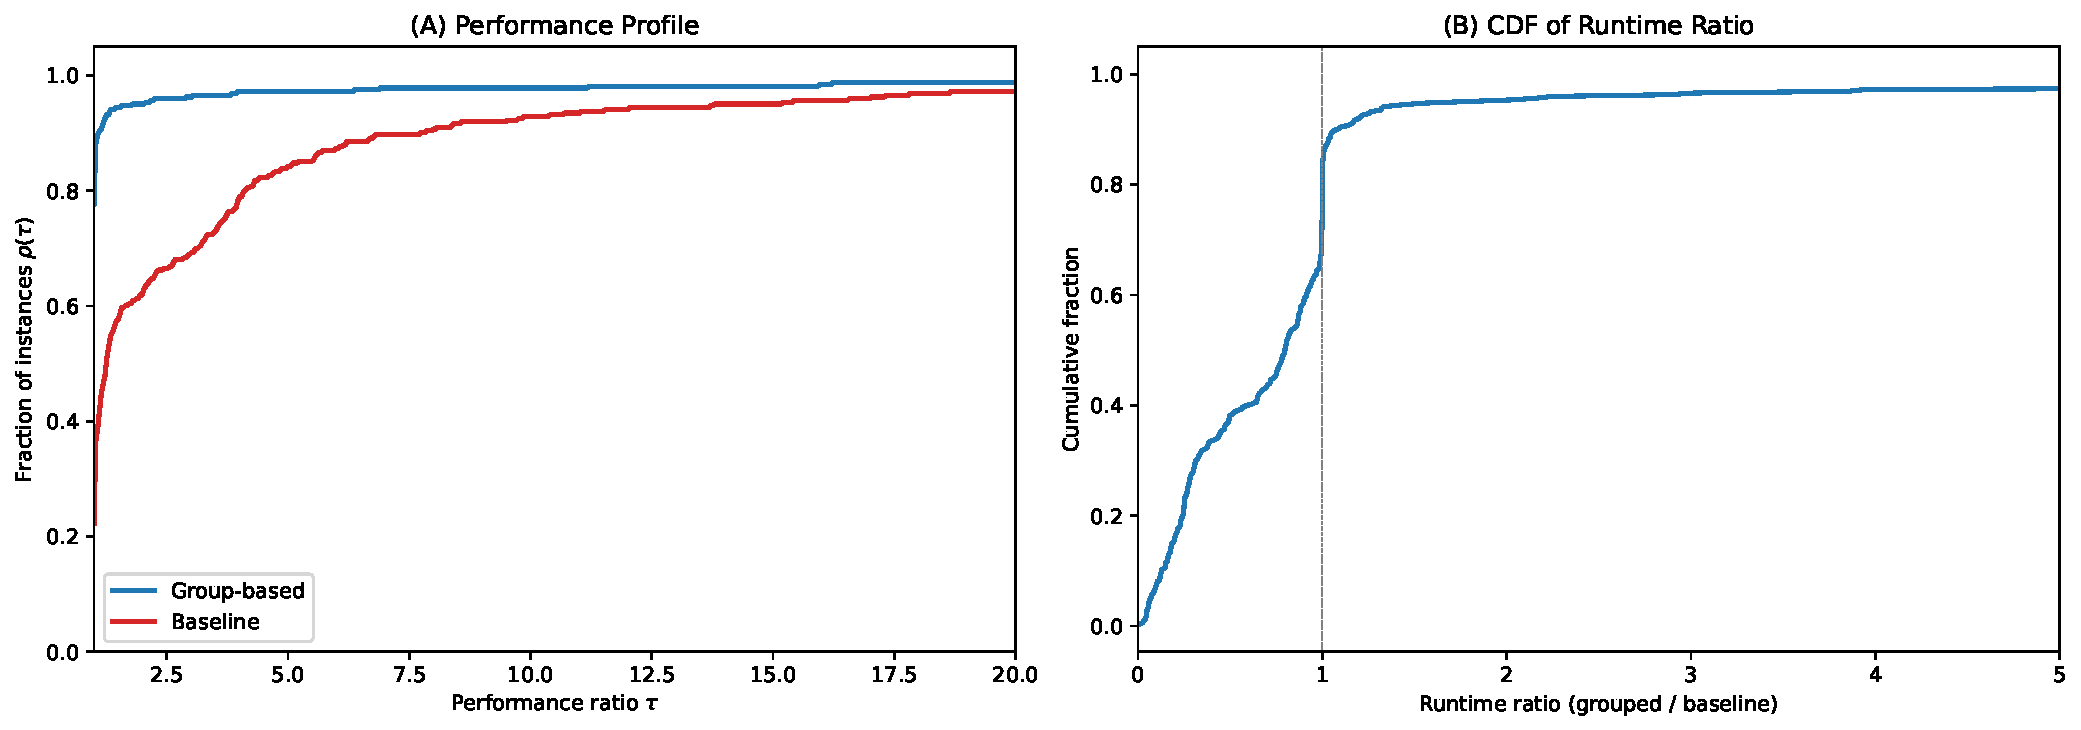
\includegraphics[width=\textwidth]{performance_profile_figure}
  \caption{Runtime comparison across all 323 jointly feasible
           instances (j10 and j30 combined).
           \textbf{(A)}~Dolan--Mor\'e performance profile:
           fraction of instances solved within a factor~$\tau$
           of the best runtime.
           \textbf{(B)}~Cumulative distribution of the runtime
           ratio (grouped~/~baseline); values below~1 indicate
           the grouped method is faster.}
  \label{fig:perf_profile}
\end{figure}
Figure~\ref{fig:gap_boxplot} shows the distribution of the
makespan gap relative to the SSGS warm-start for both methods,
broken down by~$|K|$. On j10, the distributions are nearly
identical: most instances show a gap of exactly~$0\%$ (the MIP
returns the SSGS makespan), with a few negative outliers where
the solver finds an improvement. On j30, the pattern is
similar, with median gaps of~$0\%$ for both methods at all
$|K|$ values. This confirms that the grouped method matches the
baseline in solution quality while delivering the runtime
savings documented above.
\begin{figure}[htbp]
  \centering
  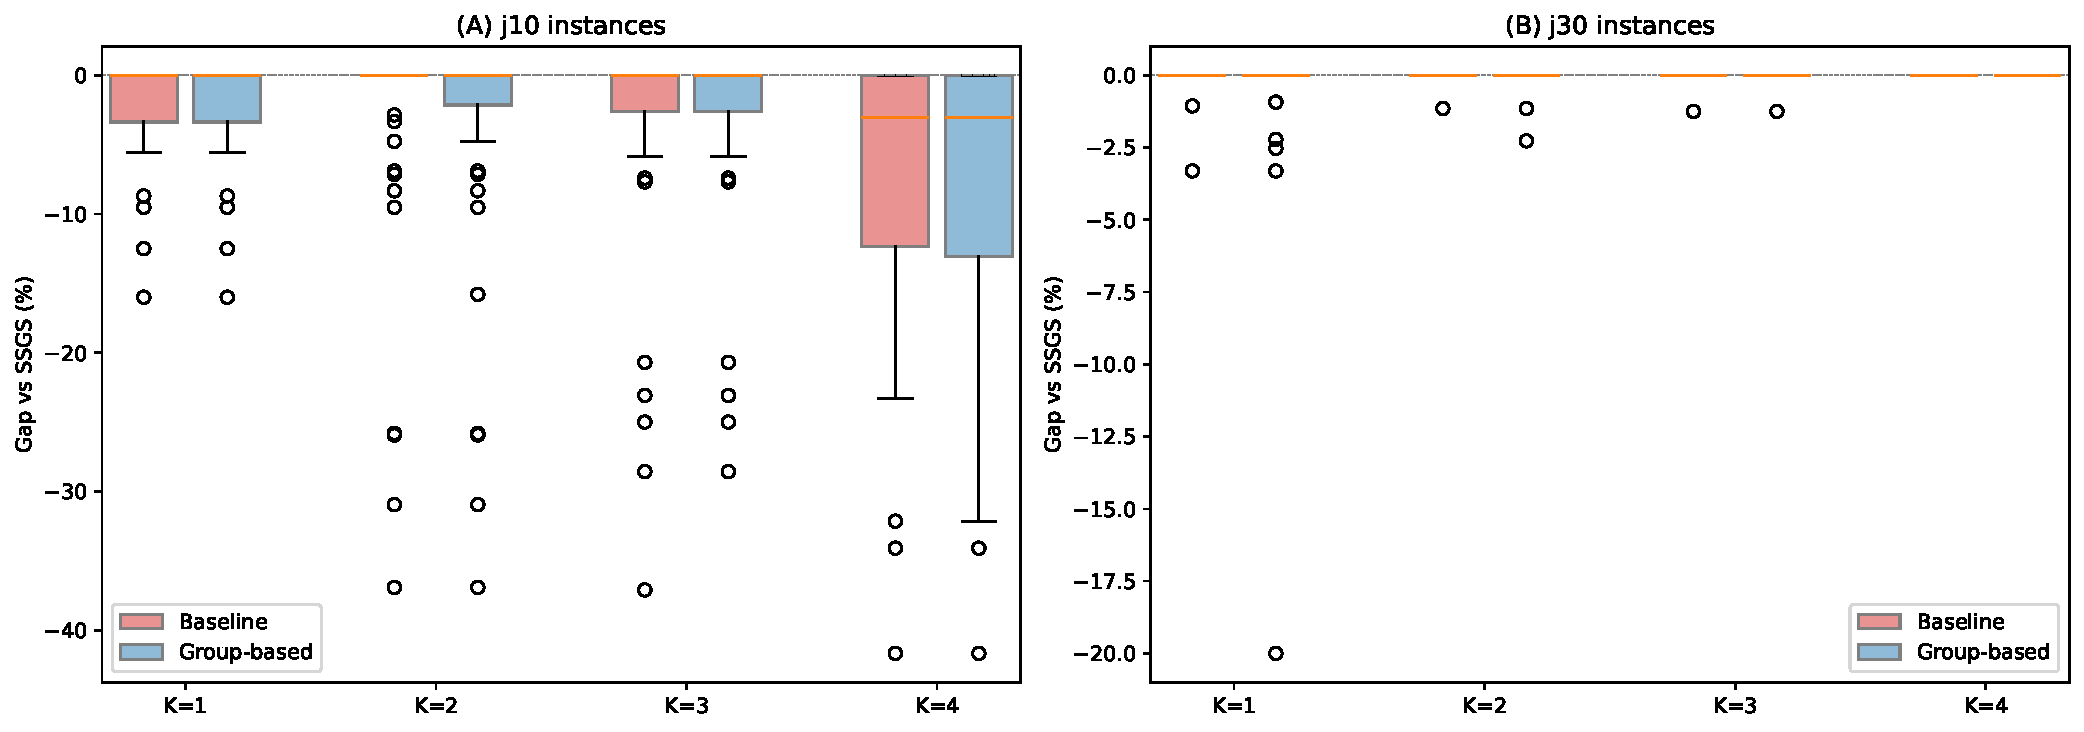
\includegraphics[width=\textwidth]{gap_boxplot_figure}
  \caption{Distribution of the makespan gap vs.\ SSGS
           warm-start (\%), grouped by~$|K|$.
           \textbf{(A)}~j10 instances.
           \textbf{(B)}~j30 instances.
           Each pair shows the baseline (red) and group-based
           (blue) R\&F on jointly feasible instances. The
           dashed line marks $0\%$ (SSGS makespan).}
  \label{fig:gap_boxplot}
\end{figure}
\subsection{Limitations}
\label{subsec:limitations}
A number of limitations apply. The stochastic workload
generator uses a fixed $\mathrm{Beta}(0.5,2.25)$ distribution
for all instances, and results may look different under
distributions with heavier tails or correlated scenarios. The
SSGS warm-start selects scenarios by aggregate workload rather
than per-resource workload, a known inconsistency discussed in
Chapter~\ref{chap:baseline}; fixing this could change the
warm-start quality and thereby shift how the two R\&F methods
compare. On the hardest j30 configuration ($|K|=4$, $|S|=10$)
without time aggregation, neither method exceeds $56\%$
feasibility; time aggregation with $\alpha=2$ brings this up to
$92\%$, but the remaining instances are still unsolved. The j60
results rely on time aggregation ($\alpha \geq 5$), which
coarsens the schedule; as
Figure~\ref{fig:alpha_sensitivity} shows, the reported gaps of
$4$--$9\%$ mix algorithmic and aggregation effects and are not
directly comparable to the j10 and j30 results. The j120
results additionally depend on per-group scenario reduction
($n_{\mathrm{keep}}=3$), introducing a further approximation
layer whose interaction with time aggregation has not been
fully characterised. Finally, all runtimes
are wall-clock measurements on a single Apple~M1 machine
running Gurobi under Rosetta~2 emulation, which means they
cannot be compared directly to results on native x86\_64
hardware in the literature.
